\section{Methods}

\subsection*{The data}

As the goal of this study is to compare some forecasts on many different pandemics, many synthetic pandemics need to be generated, with a particular attention on the diversity of these pandemics. 

\subsubsection*{Covasim}

To generate the pandemics,  \cite{kerr2021covasim}, a python librairy that can simulate the evolution of a pandemic was used. 
Covasim is an agent-based model that can model many different pandemics and has a high diversity of outputs. 
This model takes as an input many parameters such as the population type, the population size, the age repartition \dots and outputs a complete description of the pandemic, with real-time values of each relevant information, sucha as the number of severe, of asymptomatic... but also physical values such as the value of the reproduction number. 
Covasim enables to generate a huge diversity of pandemics, thanks to the plurality of parameters that can be given as the input of the model, but also with interventions that can be planned by the users. 
These interventions can simulate the impact of a vaccination campaign, with changes in the probability transmission, that can be different for all ages groups. 

\subsubsection{First pandemics}

For the implementation and the first test of the models, two pandemics were generated. 
The first one focusing on the new deaths count and the second one focusing on the number of hospitalized count. 
Those pandemics will be referred to as pandemic 1 and pandemic 2. 

\begin{table}[htbp]
    \centering
    \caption{Table of the parameters used to simulate the first two pandemics.}
    \label{tab:parameters_covasim}
    \begin{tabular}{|c|c|c|}
        \hline
        \textbf{Parameter} & \textbf{Pandemic 1} & \textbf{ Pandemic 2} \\
        \hline
        start day 1 &2020-03-02 & 2020-03-02\\
        \hline

        end day  &2020-07-01 & 2021-01-01\\
        \hline

        Population size &1000000&1000000\\
        \hline

        Interventions & interventions1 & interventions2\\
        \hline

        population type& hybrid & hybrid\\

        \hline

        $\beta$ initial &0.015 & 0.015\\
        \hline

        location & Sweden & Sweden \\
        \hline

        n infected initial &20&100\\
        \hline
    \end{tabular}
\end{table}


The parameters used to generate these pandemics are described in the table \ref{tab:parameters_covasim}.
The parameters that are not specified are the default parameters of the Covasim librairy. 


\begin{figure}
    \centering
    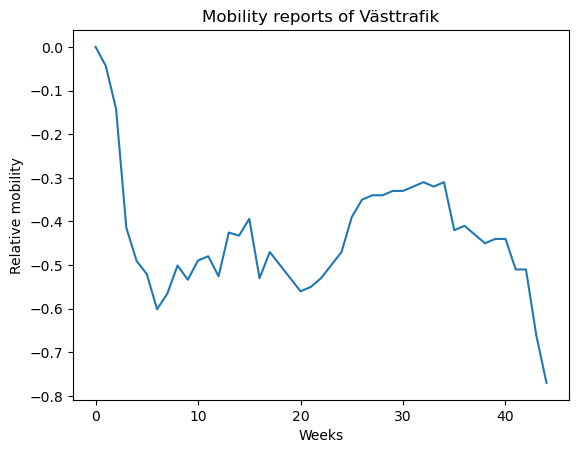
\includegraphics[width=0.8\textwidth]{figures/mobility_reports.png}
    \caption{Mobility reports from Västtrafik.}
    \label{fig:mobility_reports}
\end{figure}


The different interventions were based on mobility reports from Västtrafik  \ref{fig:mobility_reports}, the public transport company of the city of Gothenburg, which were reported during the Covid 19 pandemic and has been retrieved in \cite{gerlee2021predicting}.
These interventions correspond to 53 relative weekly variations of the mobility, with a reference value of 1 for the first week of the report, which correspond to the 9-th week of 2020. 


\subsubsection{Generating diverse pandemics}

In order to evaluate the performances of our models on a wide range of pandemics, a training set of pandemics was generated. 
A huge diversity of pandemics is needed to determine which model is the more consistent.
It is so relevant to identify the key parameters that generate this diversity.
As Covasim has a very huge set of inputs parameters, a first subset of key parameters was identified: the spread parameters and the severity parameters. 
The severity parameters are the 4 parameters that correspond to the probability for an agent to get from a compartment to another. 
The spread parameters are 9 parameters that represent the distribution of probability of the time spend by an agent in a compartment (such as infected, crictical...) once he entered it. 
This distribution is a log-normal distribution, but the spread-parameters correspond to the mean of this log-normal distribution
All the parameters have a default value of 1, which correspond to keeping the reference value. 
We decided to select 4 parameters and to make them vary in $[0.5, 1, 2]$, leading to a set of 81 pandemics. 
To select the 4 parameters that generated the most diversity, different diversity metrics were computed. 

Let $Y_1$ ,  $Y_2 \in \mathbb{R}^n$  be two time series of $n$ days representing the number of hospitalized in two pandemics.  

Let :  \\

$\mathcal{L}_1(Y_1, Y_2) = \| Y_1 - Y_2 \|_{L_1} $ \\

$\mathcal{L}_2(Y_1, Y_2) = \| (\frac{max(Y_1)}{max(Y_2)} ;\frac{max(Y_1')}{max(Y_2')} ; \frac{max(Y_1'')}{max(Y_2'')} , \| \tilde{Y_1} - \tilde{Y_2} \|_{L_1}, \| \tilde{Y_1'} - \tilde{Y_2'} \|_{L_1} , \| \tilde{Y_1''} - \tilde{Y_2''} \|_{L_1} ) \|_{L_2} $, with $Y_1$ and $Y_2$ the first and second derivatives of $Y_1$\\

It can be noted that $\mathcal{L_2}$ looks like the Sobolev norm  $\| \tilde{Y_1}  - \tilde{Y_2} \|_{W^{2, 1}} $ with squared terms and with additionary terms taking into account the amplitude. 

$\mathcal{L}_3 = \mathcal{W}(\tilde{Y_1} - \tilde{Y_2}) $, with $\mathcal{W}$ the Wasserstein distance.


$\mathcal{L}_4(Y_1, Y_2) = \| (\frac{max(Y_1)}{max(Y_2)} ;\frac{max(Y_1')}{max(Y_2')} ; \frac{max(Y_1'')}{max(Y_2'')} , \mathcal{W} (\tilde{Y_1} - \tilde{Y_2} ),\mathcal{W} ( \tilde{Y_1'} - \tilde{Y_2'} ) , \mathcal{W} (\tilde{Y_1''} - \tilde{Y_2''} ) ) \|_{L_2} $, with $Y_1$ and $Y_2$ the first and second derivatives of $Y_1$\\


To determine which measure to use, we generated 14 pandemics. Each pandemic has default parameters except one of them which was doubled, except for the last one which only have the default parameters. 

For each norm $\mathcal{L}_k$, we determined $S$,  the subset of 4 pandemics that maximized the following quantity:\\

\[ \sum_{i, j \in S, i \neq j} \mathcal{L}_k(Y_i, Y_j) \]

\begin{figure}
    \centering
    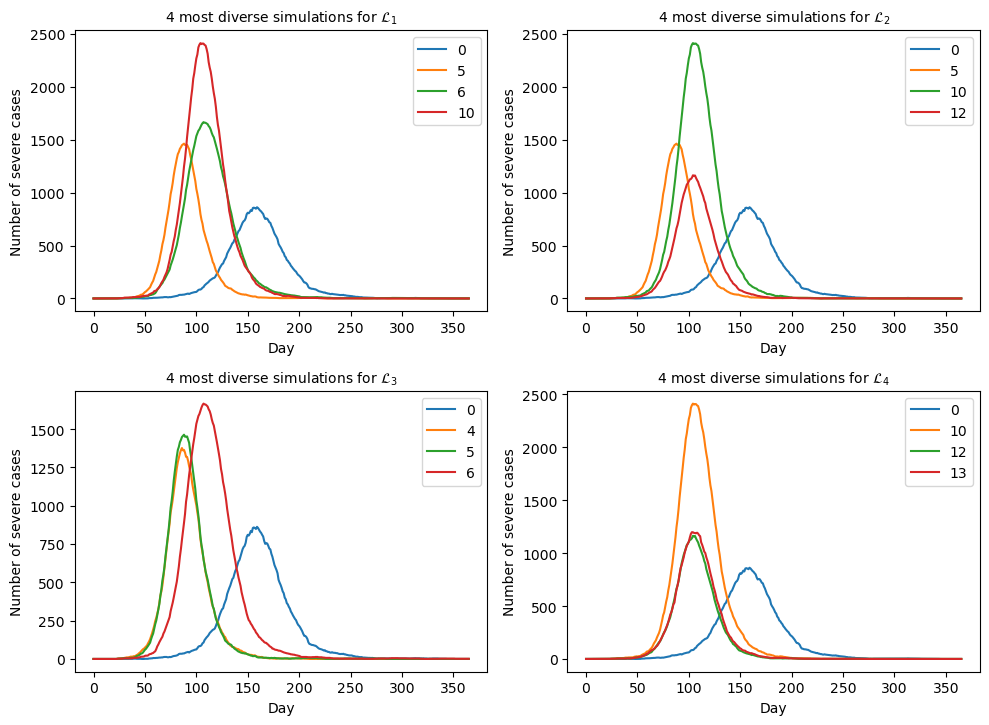
\includegraphics[width=0.8\textwidth]{figures/most_different_pandemics.png}
    \caption{4 most diverse pandemics according to each norm.}
    \label{fig:diversity_pandemics}
\end{figure}


The 4 most divers pandemics accorded to each norm are shown in the figure \ref{fig:diversity_pandemics}.
We then decided that $\mathcal{L}_2$ norm was the most relevant to determine the diversity of the pandemics.
But, keeping the parameters \texttt{[0, 5, 10, 12]} would not be relevant, the parameters were increased independantly, and the diversity did not take into account the correlation between some of them. 

Finding the parameters that maximise the $\mathcal{L}_2$ diversity is equivalent to solve the following problem : \\

$ S_{opt} = \underset{S' \subset S , \vert S' \vert =4 }{argmax} \sum_{s, t \in \mathcal{P}(S') , s \neq t }{\mathcal{L}_2(s,t)}$, with $\mathcal{P}(S')$ the set of the 81 pandemics generated with the 4 parameters of $S'$

However, generating a pandemic with \texttt{Covasim} is time consuming, and it is not possible to compute the diversity of each set of 4 parameters included inn $S$.\\[1cm]


A MCMC algorithm \cite*{diaconis2009markov} was then implemented, to perform a clever grid search on the different subsets of parameters.

\subsection{Computing confidence intervals on the prediction}

\textbf{Assumption}:
\\[0.5cm]
We suppose that the data of the pandemic observed follows the model $h$, of parameter $\theta^* \in \mathbb{R}^d$. Let $Y_i$, $ i = 1, \ldots, n$ be the number of hospitalized at each day. We suppose that: $Y_i = h_{\theta ^* } (i) + \epsilon_i$, with $\epsilon_i \sim \mathcal{N}(0, \sigma^2)$, iid, and independent from all the other variables. The objective is to estimate $\theta^*$. We use $\hat{\theta}$, the least square estimator of $\theta^*$ as an estimator of $\theta^* $:
\[
\hat{\theta} =  \underset{\theta \in \mathbb{R}^d}{\operatorname{argmin}} \sum_{i=1}^{n} (Y_i - h_{\theta}(i))^2
\]

Let:
\begin{align*}
Y &= \begin{pmatrix}
Y_1 \\
\vdots \\
Y_n
\end{pmatrix} \\
h_\theta &= \begin{pmatrix}
h_\theta(1) \\
\vdots \\
h_\theta(n)
\end{pmatrix}
\end{align*}

We have:
\[
\hat{\theta} =  \underset{\theta \in \mathbb{R}^d}{\operatorname{argmin}}  \left\lVert Y - h_\theta \right\rVert ^2
\]

Now, if $\theta$ is close enough to $\theta^*$, we can write:
\[
\forall i \in \{ 1, ..., n\} :  h_\theta(i) = h_{\theta^*} (i ) + (\theta - \theta^*)^T\nabla_\theta h_{\theta^*}(i) 
\]
which leads to:
\[
\hat{\theta} =  \underset{\theta \in \mathbb{R}^d}{\operatorname{argmin}}  \left\lVert Y - h_{\theta^*}  - (\theta - \theta^*)^T\nabla_\theta h_{\theta^*}\right\rVert ^2
\]

Let us define:
\begin{align*}
\tilde{Y} &= Y - h_{\theta^*} \\
\beta &= \theta - \theta^* \\
\hat{\beta} &= \theta - \hat{\theta}
\end{align*}

and let us define the matrix $A \in \mathbb{R} ^{n \times d }$ such that $\forall i \in \{ 1, ..., n\}, \forall j \in \{1, ..., d\}, A_{i, j} = \frac{dh_{\theta^*}}{d\theta_j}(i)$.

The previous problem can be re-written as:
\[
\hat{\beta} =  \underset{\beta \in \mathbb{R}^d}{\operatorname{argmin}}  \left\lVert \tilde{Y} - A \beta \right\rVert ^2
\]

This is a regression linear problem.

Let us solve this problem in the general case.

Let $(A_i, \tilde{Y_i})$ be the observations Let $\mathbb{P}$ be the law of $A_i$, and let us assume that $Y_i = A_i \beta ^* + \epsilon_i $, with $\epsilon_i \sim \mathcal{N}(0, \sigma^2)$.

% Let  $\tilde{Y}_i = A_i \beta ^* + \epsilon'_i $, with  $\epsilon'_i \sim \mathcal{N}(0, \sigma ' ^2)$.

The solution of this problem is explicitly:
\[
\hat{\beta } = (A^T A ) ^{-1} A^T \tilde{Y}
\]

This least-square estimator is unbiased:
\[
\mathbb{E}[\hat{\beta}] = \beta^*
\]

\[
\hat {\beta } = \left(  \sum_{i=1}^{n}   A_i ^T A_i \right) ^{-1}    \times \left(  \sum_{i=1}^{n} A_i ^T \tilde{Y_i } \right)
\]

\[
\hat {\beta } =\frac{n}{n} \left(  \sum_{i=1}^{n}   A_i ^T A_i \right) ^{-1}    \times \left(  \sum_{i=1}^{n} A_i ^T \tilde{Y_i } \right)
\]

\[
\hat {\beta } = \left( \frac{1}{n} \sum_{i=1}^{n}   A_i ^T A_i \right) ^{-1}    \times \left( \frac{1}{n} \sum_{i=1}^{n} A_i ^T \tilde{Y_i } \right)
\]

Let us denote:
\[
\hat{D}  = \frac{1}{n} \sum_{i=1}^{n}   A_i ^T A_i , \quad \text{and} \quad \hat{\delta}  = \left( \frac{1}{n} \sum_{i=1}^{n} A_i ^T \tilde{Y_i } \right)
\]

We have:
\[
\hat{\beta} = \hat{D} ^{-1} \hat{\delta}
\]

\[
\hat{D}  \underset{a.s}{\rightarrow} D=  \mathbb{E}[A_i ^T A_i ]
\]

\[
\hat{\delta}   \underset{a.s}{\rightarrow}  \delta = \mathbb{E}[A_i ^T \tilde{Y}_i ]
\]

$ \hat{\beta} = \hat{D}^{-1} \hat{\delta}  \underset{a.s}{\rightarrow}  D^{-1} \delta $ , as the following function $\phi$ is continuous:
\[
\phi: \left\{
\begin{array}{rcl}
\mathcal{GL}_n(\mathbb{R}) & \to & \mathcal{GL}_n(\mathbb{R}) \\
A & \mapsto & A^{-1}
\end{array}
\right.
\]




Now, let us show that $\hat{\beta}$ is asymptotically normal: 

\begin{align*}
    \sqrt{n} ( \hat{\beta} - \beta ^* ) &= \sqrt{n} (\hat{D}^{-1} \hat{\delta} - \beta ^* ) \\
     &= \sqrt{n} (\hat{D}^{-1} \hat{\delta} - \hat{D}^{-1} \hat{D} \beta ^* ) \\
     &= \sqrt{n} \hat{D}^{-1} (\hat{\delta} -  \hat{D} \beta ^* )  \\
     &= \sqrt{n} \hat{D}^{-1} \left( \frac{1}{n} \sum_{i=1}^{n} A_i ^T \tilde{Y_i} - \frac{1}{n}  \sum_{i=1}^{n}  A_i ^T A_i \beta ^* \right)  \\
     &= \frac{\sqrt{n}}{n} \hat{D}^{-1} \left( \sum_{i=1}^{n} A_i ^T (\tilde{Y_i} -    A_i \beta ^* ) \right)   \\
     &= \frac{1}{\sqrt{n}}  \hat{D} ^{-1} \left( \sum_{i=1}^{n}  A_i ^T \epsilon _ i \right)  
\end{align*}

This line is made of two terms. Let's show that each one of them converges in law. 

\begin{align*}
    \frac{1}{\sqrt{n}} \left( \sum_{i=1}^{n}  A_i^T \epsilon'_i \right) &= \sqrt{n} \left( \frac{1}{n} \sum_{i=1}^{n}  A_i^T \epsilon'_i \right) \\
    &= \sqrt{n} \left( \frac{1}{n} \sum_{i=1}^{n}  A_i^T \epsilon'_i - 0 \right) \\
    &\xrightarrow{\mathcal{L}} \mathcal{N}(0, \text{Var}(A_i^T \epsilon_i) )
\end{align*}

Yet, as $\epsilon_i $ and $  A_i $ are independant, and $\mathbb{E} [ A_i^T \epsilon'_i] = 0 $ , $\text{Var}(A_i^T \epsilon_i) = \mathbb{E}[A_i A_i ^T \epsilon_i ^2 ] = \mathbb{E} [ A_i A_i ^T ] \sigma'^2$. 

Finally, $\frac{1}{\sqrt{n}} \left( \sum_{i=1}^{n}  A_i^T \epsilon'_i \right) \xrightarrow{\mathcal{L}} \mathcal{N}(0, D \sigma'^{2})$. 

On the other hand, $\hat{D}^{-1} \xrightarrow{\mathcal{L}} D^{-1} $, which is constant.

Finally, with Slutsky, we obtain that: 

\begin{align*}
    \sqrt{n} (\hat{\beta} - \beta^*) &\xrightarrow{\mathcal{L}} D^{-1}\mathcal{N}(0, D \sigma'^2) \\
    &\xrightarrow{\mathcal{L}} \mathcal{N}(0, D^{-1} (D \sigma'^2) (D^{-1})^T) \\
    &\xrightarrow{\mathcal{L}} \mathcal{N}(0, D^{-1} D \sigma'^2 (D^{-1})^{T}) \\
    &\xrightarrow{\mathcal{L}} \mathcal{N}(0, \sigma'^2 D^{-1}) \\
    &\xrightarrow{\mathcal{L}} \mathcal{N}(0, \sigma'^2 (A^T A)^{-1})
\end{align*}


Let's get back to the first problem: 

As $\beta ^* = 0 $ and $\hat{\beta} = \hat{\theta} - \theta ^* $, we have: 

\[
\sqrt{n} (\hat{\theta} - \theta^*) \xrightarrow{\mathcal{L}} \mathcal{N}(0, \sigma^2 (A^T A)^{-1})
\]

and, 
\[
\hat{\theta} \sim \mathcal{N}(\theta^*, \frac{\sigma^2}{n} (A^T A)^{-1})
\]

As a first conclusion, we have that $\hat{\theta}$ is asymptotically normal.

Let $\Sigma$ be the covariance matrix estimated from the computation of $\hat{\theta}$. In our case, $\Sigma = \frac{\sigma^2}{n} (A^T A)^{-1}$. 

As $\hat{\theta}$ is asymptotically normal, we can apply the delta-method: 

\[
\sqrt{n} (\hat{\theta} -\theta^*) \xrightarrow{\mathcal{L}} \mathcal{N}(0, \ \Sigma)
\]
\[
\sqrt{n} (h_{\hat{\theta}} -h_{\theta^*}) \xrightarrow{\mathcal{L}} \mathcal{N}(0, \nabla_\theta h_\theta ^T \Sigma  \nabla_\theta h_\theta)
\]

And finally: 
\[
h_{\hat{\theta}} \rightarrow \mathcal{N}(h_{\theta^*}, \frac{1}{n}\nabla_\theta h_\theta ^T \Sigma  \nabla_\theta h_\theta)
\]

By estimating $\frac{1}{n} \Sigma$ from \texttt{curve\_fit}, we can compute the confidence interval of the prediction with the quantiles of the normal distribution.
